\documentclass[a4paper,12pt]{article}

\usepackage[T2A]{fontenc}			
\usepackage[utf8]{inputenc}			
\usepackage[english,russian]{babel}	

\usepackage[
bookmarks=true, colorlinks=true, unicode=true,
urlcolor=black,linkcolor=black, anchorcolor=black,
citecolor=black, menucolor=black, filecolor=black,
]{hyperref}

\usepackage{color}
\usepackage{caption}
\DeclareCaptionFont{white}{\color{black}}
\DeclareCaptionFormat{listing}{\colorbox{white}{\parbox{\textwidth}{#1#2#3}}}
\captionsetup[lstlisting]{format=listing,labelfont=white,textfont=white}

\usepackage{amsmath,amsfonts,amssymb,amsthm,mathtools} 
\usepackage{wasysym}

\usepackage{graphicx}
%\usepackage[cache=false]{minted}
\usepackage{cmap}
\usepackage{indentfirst}

\usepackage{listings} 
\usepackage{fancyvrb}

\usepackage{geometry}
\geometry{left=2cm}
\geometry{right=1.5cm}
\geometry{top=1cm}
\geometry{bottom=2cm}

\setlength{\parindent}{5ex}
\setlength{\parskip}{0.5em}

\usepackage{pgfplots}
\usetikzlibrary{datavisualization}
\usetikzlibrary{datavisualization.formats.functions}

\begin{filecontents}{Machinee.dat}
	10 0.000038
	20 0.000056
	30 0.000064
	40 0.000072
	50 0.000081
	60 0.000157
	70 0.000104
	80 0.000092
	90 0.000148
	100 0.000156
\end{filecontents}

\begin{filecontents}{Regularr.dat}
	10 0.000588
	20 0.000516
	30 0.000642
	40 0.000564
	50 0.000641
	60 0.000665
	70 0.000650
	80 0.000632
	90 0.000833
	100 0.000624
\end{filecontents}

\begin{document}
	\lstset{ %
		language=Python,                 % выбор языка для подсветки (здесь это С)
		basicstyle=\small\sffamily, % размер и начертание шрифта для подсветки кода
		numbers=left,               % где поставить нумерацию строк (слева\справа)
		numberstyle=\tiny,           % размер шрифта для номеров строк
		stepnumber=1,                   % размер шага между двумя номерами строк
		numbersep=5pt,                % как далеко отстоят номера строк от подсвечиваемого кода
		backgroundcolor=\color{white}, % цвет фона подсветки - используем \usepackage{color}
		showspaces=false,            % показывать или нет пробелы специальными отступами
		showstringspaces=false,      % показывать или нет пробелы в строках
		showtabs=false,             % показывать или нет табуляцию в строках
		frame=single,              % рисовать рамку вокруг кода
		tabsize=2,                 % размер табуляции по умолчанию равен 2 пробелам
		captionpos=t,              % позиция заголовка вверху [t] или внизу [b] 
		breaklines=true,           % автоматически переносить строки (да\нет)
		breakatwhitespace=false, % переносить строки только если есть пробел
		escapeinside={\%*}{*)}   % если нужно добавить комментарии в коде
	}

% Титульный лист
\large
\begin{center}
	Федеральное государственное бюджетное образовательное учреждение 
	высшего образования <<Московский государственный технический 
	университет имени Н. Э. Баумана>> 
	(национальный исследовательский университет)
\end{center}

\vspace*{30mm} 

\huge
\begin{center}
	Дисциплина: <<Анализ алгоритмов>>
	
	Отчет по рубежному контролю №2
\end{center}

\vspace*{30mm} 

\huge
\begin{center}
	Тема работы:\\
	<<Конечные автоматы.\\ Регулярные выражения>>
\end{center}
\vspace*{30mm} 

\large
\begin{flushright}
	Студент: Левушкин И. К. \\
	Группа: ИУ7-52Б \\
	Преподаватели: Волкова Л. Л., \\ Строганов Ю. В. \\
\end{flushright}

\vspace*{40mm}
\begin{center}
	Москва, 2019 г.  
\end{center}
\thispagestyle{empty}

\tableofcontents

\section*{Введение}
\addcontentsline{toc}{section}{Введение}

\textbf{Цель лабораторной работы:} При помощи конечных автоматов и регулярных выражений написать программу, находящую группы факультетов ИУ, ИБМ и Э в тексте.

\textbf{Задачи работы:}

\begin{enumerate} 
	\item[1)] изучить работу регулярных выражений и конечных автоматов;
	\item[2)] создать конечный автомат;
	\item[3)] реализовать поставленную задачу с использованием конечного автомата;
	\item[4)] реализовать поставленную задачу с использованием регулярные выражения;
	\item[5)] сравнить время выполнения программы, использующую конечный автомат, и программу, использующую регулярные выражения;
	\item[6)] описать и обосновать полученные результаты в отчете о рубежном контроле 
	работе, выполненного как расчётно-пояснительная записка. 
\end{enumerate} 
\pagebreak

\section{Аналитический раздел}

\subsection{Конечные автоматы}

Конечный автомат (или попросту FSM — Finite-state machine) это модель вычислений, основанная на гипотетической машине состояний. В один момент времени только одно состояние может быть активным. Следовательно, для выполнения каких-либо действий машина должна менять свое состояние.
Конечные автоматы обычно используются для организации и представления потока выполнения чего-либо.
Конечный автомат можно представить в виде графа, вершины которого являются состояниями, а ребра — переходы между ними. Каждое ребро имеет метку, информирующую о том, когда должен произойти переход.

\subsection{Регурярные выражения}

Регулярные выражения – это алгебраический способ описания
регулярных языков, которые задают конечные автоматы.
Алгебраическими регулярными операторами являются:
объединение, конкатенация (“точка”) и итерация
(“звездочка”).

Регулярные выражения подчиняются многим алгебраическим
законам арифметики, хотя есть и различия. Объединение и
конкатенация ассоциативны, но только объединение
коммутативно. Конкатенация дистрибутивна относительно
объединения. Объединение идемпотентно.

\section{Конструкторский раздел}

В разделе представлен конечный автомат для реализации задачи нахождения всех групп факультетов ИУ, ИБМ и Э в тексте.

На рисунке \ref{ris:machine} приведен конечный автомат для поставленной задачи.

\begin{figure}[h!]
	\begin{center}
		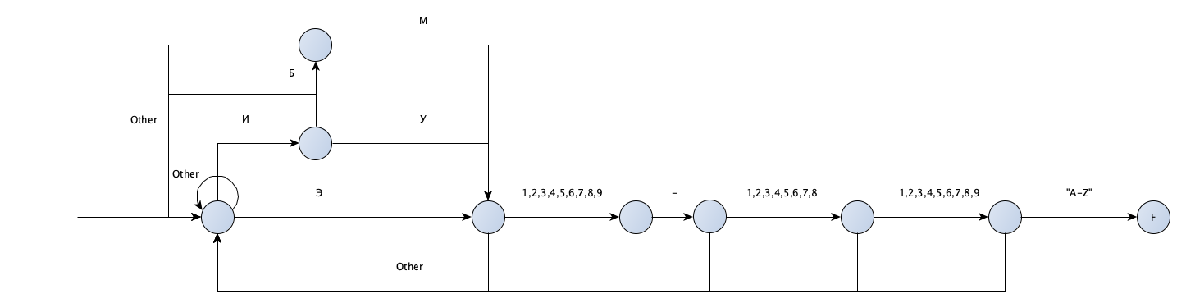
\includegraphics[scale = 0.65]{machine.pdf}
		\caption{Конечный автомат для определения группы факультетов ИУ, ИБМ, Э}
		\label{ris:machine}
	\end{center}
\end{figure}


\section{Технологический раздел}

Здесь описываются требования к программному 
обеспечению и средства реализации, приводятся листинги 
программы и тестовые данные.

\subsection{Требования к программному обеспечению}

\begin{flushleft}
	\textbf{Входные данные:} 
	\begin{itemize}
		\item строка символов.
	\end{itemize}
	
	\textbf{Выходные данные:} словарь, хранящий в качестве ключа позицию группы в данном тексте, а в качестве значения - саму группу.
\end{flushleft}

\subsection{Средства реализации}

Программа написана на языке Python ~\cite{python}, который 
предоставляет программисту мощные инструменты для реализации различных алгоритмов и является достаточно 
надежным, эффективным и удобным для реализации сложных алгоритмов. Для написания использовался 
редактор исходного кода \textit{PyCharm} ~\cite{pycharm}.

Замер времени выполнения программы 
производится с помощью функции \textit{process\_time()} из библиотеки \textit{time},
функционал которой позволяет подсчитывать процессорное время в тиках,
а затем конвертировать полученный результат в секунды.

\subsection{Листинг программы}

Реализованная программа представлена
в листингах \ref{lst1}-\ref{lst2}.

\begin{lstlisting}[label=lst1,caption=Реализация программы с использованием регулярных выражений]
import re

def regular(line):
	result = re.findall(r'(?:IU|IBM|E)[1-9]-[1-8][1-9][A-Z]', line)
	return result
\end{lstlisting}

\begin{lstlisting}[label=lst2,caption=Реализация программы с применением конечного автомата]
def machine(line):
	result = {}
	faculty = ''
	state = 0
	state_3_choice = [1,2,3,4,5,6,7,8,9]
	state_5_choice = [1,2,3,4,5,6,7,8]
	state_6_choice = [1,2,3,4,5,6,7,8,9]
	state_7_choice = [A-Z]
	for i in range(len(line)):
		if (state == 0):
			if (line[i] == 'I'):
				state = 1
				faculty += line[i]
			elif (line[i] == 'E'):
				state = 3
				faculty += line[i]
			else:
				continue
		elif (state == 1):
			if (line[i] == 'B'):
				state = 2
				faculty += line[i]
			elif (line[i] == 'U'):
				state = 3
				faculty += line[i]
			else:
				faculty = ''
				state = 0
				i -= 1
		elif (state == 2):
			if (line[i] == 'M'):
				state = 3
				faculty += line[i]
			else:
				faculty = ''
				state = 0
				i -= 1
		elif (state == 3):
			if (int(line[i]) in state_3_choice):
				state = 4
				faculty += line[i]
			else:
				faculty = ''
				state = 0
				i -= 1
		elif (state == 4):
			if (line[i] == '-'):
				faculty += line[i]
				state = 5
			else:
				faculty = ''
				state = 0
				i -= 1
		elif (state == 5):
			if (int(line[i]) in state_5_choice):
				state = 6
				faculty += line[i]
			else:
				faculty = ''
				state = 0
				i -= 1
		elif (state == 6):
			if (int(line[i]) in state_6_choice):
				state = 7
				faculty += line[i]
			else:
				faculty = ''
				state = 0
				i -= 1
		elif (state == 7):
		if (line[i] in state_7_choice):
			faculty += line[i]
			result.update({i - len(faculty) + 1: faculty})
			state = 0
			faculty = ''
		else:
			faculty = ''
			state = 0
			i -= 1
	return result
\end{lstlisting}

\section{Исследовательский раздел}

В разделе представлены примеры выполнения программы,
результаты сравнения времени выполнения программ, реализованных на конечных автоматах и с использованием регулярных выражений.

\subsection{Примеры работы}

На рис. \ref{fig:t0}-\ref{fig:t4} приведены примеры работы программы. 

\newpage

\begin{figure}[h!]
	\center{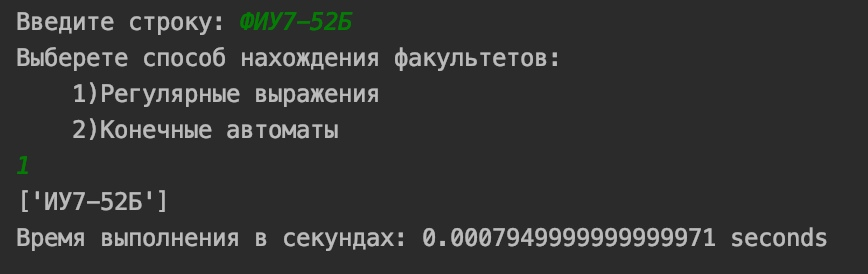
\includegraphics[scale = 0.65]{0.jpg}}
	\caption{
		Пример работы регулярных выражений}
	\label{fig:t0}
\end{figure}

\begin{figure}[h!]
	\center{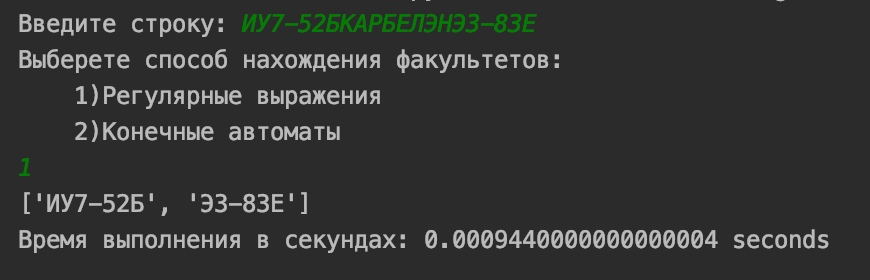
\includegraphics[scale = 0.65]{1.jpg}}
	\caption{
		Пример работы регулярных выражений}
	\label{fig:t1}
\end{figure}

\begin{figure}[h!]
	\center{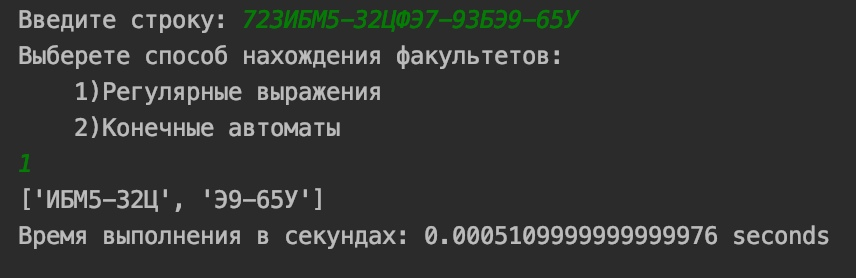
\includegraphics[scale = 0.65]{2.jpg}}
	\caption{
		Пример работы регулярных выражений}
	\label{fig:t2}
\end{figure}

\newpage

\begin{figure}[h!]
	\center{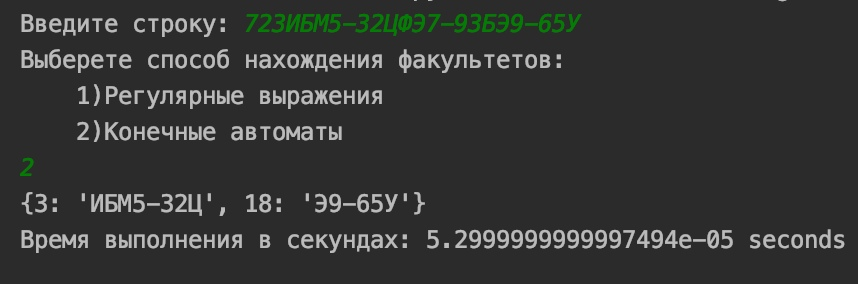
\includegraphics[scale = 0.65]{3.jpg}}
	\caption{
		Пример работы конечного автомата}
	\label{fig:t3}
\end{figure}

\begin{figure}[h!]
	\center{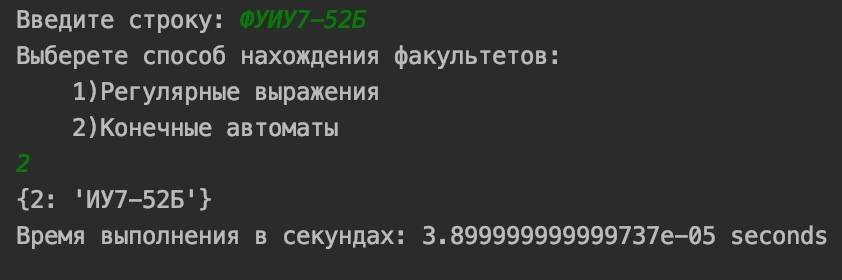
\includegraphics[scale = 0.65]{4.jpg}}
	\caption{
		Пример работы конечного автомата}
	\label{fig:t4}
\end{figure}

\subsection{Постановка эксперимента}

\begin{enumerate}
	\item Сравнить время работы алгоритма, разработанного на основе конечного автомата и алгоритма с использованием регулярных выражений на строке длинной 10-100 символов с шагом в 10 символов.
\end{enumerate}

\subsection{Тестовые данные}

Строки будут состоять из следующих символов:
\begin{enumerate}
	\item $str10$ : \textit{уюмЭ7-52Бв};
	\item $str20$ : \textit{уюмЭ7-52БИУ3-21Ее4К6};
	\item $str30$ : \textit{уюмЭ7-52БИУ3-21Ее4К6Э5-32Кпртры};
	\item $str40$ : \textit{уюмЭ7-52БИУ3-21Ее4К6Э5-32КпртрыИБМ4-19Цепу};
	\item $str50$ : \textit{уюмЭ7-52БИУ3-21Ее4К6Э5-32КпртрыИБМ4-19ЦепуЭ5-32К};
	\item $str60$ : \textit{уюмЭ7-52БИУ3-21Ее4К6Э5-32КпртрыИБМ4-19ЦепуЭ5-32КИУ9-61У};
	\item $str70$ : \textit{уюмЭ7-52БИУ3-21Ее4К6Э5-32КпртрыИБМ4-19ЦепуЭ5-32КИУ9-61УИБМ4-19Ц};
	\item $str80$ : \textit{уюмЭ7-52БИУ3-21Ее4К6Э5-32КпртрыИБМ4-19ЦепуЭ5-32КИУ9-61УИБМ4-19ЦИБМ4-19Цапывы};
	\item $str90$ : \textit{уюмЭ7-52БИУ3-21Ее4К6Э5-32КпртрыИБМ4-19ЦепуЭ5-32КИУ9-61УИБМ4-19ЦИБМ4-19ЦИУ9-61УЭ5-32КИУ9-61Уиа};
	\item $str100$ : \textit{уюмЭ7-52БИУ3-21Ее4К6Э5-32КпртрыИБМ4-19ЦепуЭ5-32КИУ9-61УИБМ4-19ЦИБМ4-19ЦИУ9-61УЭ5-32КЭ5-32КИУ9-61УИУ9-61Уйц}.
\end{enumerate}


\subsection{Сравнительный анализ на основе эксперимента}

\subsubsection{Сравнение времени работы}

Замеры произведены на 4-ядерном процессоре \textit{Intel Core i7}
с тактовой частотой 2,4 ГГц, оперативная память --- 8 ГБ.

Экспериментально получена таблица сравнения времени 
(табл. \ref{time1}, время в секундах (с)):

\begin{table} [h!]
	\begin{center}
		\caption{Сравнение времени выполнения алгоритмов на основе конечных автоматов и с использованием регулярных выражений}
		\begin{tabular}{|r|r|r|}
			\hline
			Длина слова & Конечный автомат, с & Регулярные выражения, с \\
			\hline
			10 &    0.000038 &   0.000588 \\
			\hline
			20 &    0.000056 &   0.000516 \\
			\hline
			30 &    0.000064 &   0.000642 \\
			\hline
			40 &    0.000072 &   0.000564 \\
			\hline
			50 &    0.000081 &   0.000641 \\
			\hline
			60 &    0.000157 &   0.000665 \\
			\hline
			70 &    0.000104 &   0.000650 \\
			hline
			80 &    0.000092 &   0.000632 \\
			\hline
			90 &    0.000148 &   0.000833 \\
			\hline
			100 &  0.000156 &   0.000624 \\
			\hline
		\end{tabular} 
		\label{time1}
	\end{center}
\end{table}

\newpage

Ниже полученные данные представлены в виде графика:

\begin{figure}[h!]
	\centering
\begin{tikzpicture}
	\begin{axis}[
	axis lines = left,
	xlabel = {$symbols$, символов},
	ylabel = {$time$, секунд},
	legend pos=north west,
	ymajorgrids=true
	]
	\addplot[color=red] table[x index=0, y index=1] {Machinee.dat};
	\addplot[color=green, mark=square] table[x index=0, y index=1] {Regularr.dat};
	
	\addlegendentry{Machine}
	\addlegendentry{Regular}
	
	\end{axis}
\end{tikzpicture}
\caption{График зависимости времени работы алгоритмов от количества символов в строке}
\end{figure}

Видно, что алгоритм, основанный на конечных автоматах, в среднем затрачивает в 10 раз меньше времени на поиск групп факультетов нежели алгоритм использующий регулярные выражения.



\section{Выводы по экспериментальному разделу}

~\

В данном разделе было проведено исследование временных затрат разработанного программного обеспечения, вместе с сравнительным анализом реализованных алгоритмов на основе экспериментальных данных. В результате проведенного исследования выяснилось, что алгоритм, основанный на конечных автоматах, в среднем затрачивает в 10 раз меньше времени на поиск групп факультетов нежели алгоритм использующий регулярные выражения, что напрямую вытекает из теоретического материала приведенного в аналитическом разделе.

\section*{Заключение}
\addcontentsline{toc}{section}{Заключение}

~\

В ходе выполнения данной лабораторной работы были изучены конечные автоматы и регулярные выражения. Алгоритмы были разработаны и реализацованы, было проведено исследование временных затрат алгоритмов, а
также дано описание и обоснование полученных результатов.

\newpage

\addcontentsline{toc}{section}{Список литературы}
\begin{thebibliography}{}

	\bibitem{python}
	Python 3.8.2rc1 documentation [Электронный ресурс]. - Режим доступа: https://docs.python.org/3/, свободный - (28.11.2019)
	
	\bibitem{pycharm}
	PyCharm documentation [Электронный ресурс]. - Режим доступа: https://www.jetbrains.com/pycharm/documentation/ - (28.11.2019)

\end{thebibliography}

\end{document}